\rhead{29 January 2018}

\begin{Bsp}
Let $k = \C$, $I=(Y^2-X(X-1)(X-\lambda))$ with $\lambda \in \C$ and $V=V(I)$.
Observe that $I$ is a prime ideal since $f_\lambda$ is irreducible (use Eisenstein criterion). In particular, $I=I(V)$. Hence $V$ is irreducible and
\[ K[V] = k[X,Y] / I.\]

Graph for $\lambda = -1$:
\[ 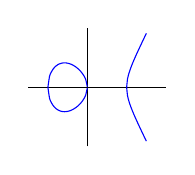
\begin{tikzpicture}[scale=0.5]
\draw(-1.5,0) -- (2,0);
\draw(0,-1.5) -- (0,1.5);
\draw[smooth, domain=-1:0, variable=\x,blue] plot ({\x},{sqrt(\x*\x*\x-\x)});
\draw[smooth, domain=1:1.5, variable=\x,blue] plot ({\x},{sqrt(\x*\x*\x-\x)});
\draw[smooth, domain=-1:0, variable=\x,blue] plot ({\x},{-sqrt(\x*\x*\x-\x)});
\draw[smooth, domain=1:1.5, variable=\x,blue] plot ({\x},{-sqrt(\x*\x*\x-\x)});
\end{tikzpicture}
\]
\end{Bsp}

\begin{defi}
\begin{enumerate}[(i)]
\item Let $X$ be a topological space. The \textbf{Krull dimension} $\dim(X)$ of $X$ is defined as
\begin{align*}
	\dim(X) = \sup \{ n \in \N \, | \, &\text{there are closed, irreducible subsets } X_i \subset X \text{ with } \\
	&\emptyset \neq X_0 \subsetneq X_1 \subsetneq \cdots \subsetneq X_n \}.
\end{align*}
\item Let $R$ be an arbitrary commutative noetherian ring. Then
\begin{align*}
\dim(R) = \sup \{ n \in \N \, | \, &\text{there are  } \p_i \in \Spec R \text{ with } 
 \p_0 \supsetneq \p_1 \supsetneq \cdots \supsetneq \p_n \}.
\end{align*}
is called the \textbf{dimension} of $R$.
\end{enumerate}
\end{defi}

\begin{Bem}
	By Conclusion 2.20 we have $\dim V = \dim k[V]$.
\end{Bem}

\begin{Fakt}
	$\dim k[X_1, \dots, X_n] =n$ and hence $\dim \Aff^n(k) = n$.
\end{Fakt}


\begin{Beob*}
	$ (X_1, \dots, X_n) \supsetneq (X_1, \dots, X_{n-1} )\supsetneq \cdots \supsetneq (X_1) \supsetneq (0)$
	is a chain of prime ideals of length $n$, hence $\dim k[X_1, \dots, X_n] \geq n$.
	
	But you have to do some work to show that there is not a longer one.
\end{Beob*}

\begin{Bsp}
Let $V=V((f_\lambda))$ with $f_\lambda = Y^2-X(X-1)(X-\lambda)$ and observe that
$\p_0 =(X,Y) \supsetneq \p_1 =(f_\lambda) = I$ in $k[X,Y]$ induces
$\overline{\p}_0 \supsetneq \overline{\p}_1$ in $ k[V] = k[X,Y] / I$, where $\overline{\p}_i$ is the image of $p_i$ in the quotient. Hence $\dim k[V] \geq 1$.

But any chain of prime ideals $\overline{\p}_0 \supsetneq \overline{\p}_1 \supsetneq \cdots \supsetneq \overline{\p}_n =(0) $ of length $n$  in $k[V]$ induces a chain of prime ideals 
${\p}_0 \supsetneq {\p}_1 \supsetneq \cdots \supsetneq {\p}_n \supsetneq (0) $ 
of length $N+1$, where $\p_i$ is the preimage of $\overline{\p}_i$.
Hence, by Fact 2.24, $\dim k[V] = 1$.
\end{Bsp}

\begin{defi}
An \textbf{affine curve} over $k$ is an irreducible affine variety $V$ over $k$ of dimension $1$.
\end{defi}


\begin{defi}
Let $V \subset \Aff^n(k)$ be an irreducible affine variety of dimension $d$ with $V=V(f_1,\dots,f_r)$.
For $z \in V$ consider the Jacobian matrix
\[ J = \left( \frac{\partial f_i}{\partial x_j} (z)  \right) = \begin{pmatrix}
\frac{\partial f_1}{\partial x_1} (z) & \cdots & \frac{\partial f_1}{\partial x_n} (z) \\
\vdots & \ddots & \vdots \\
\frac{\partial f_r}{\partial x_1} (z) & \cdots & \frac{\partial f_r}{\partial x_n} (z) \\
\end{pmatrix}.
\]
In this case,
\begin{itemize}
	\item $z\in V$ is called \textbf{singular} if $\rank J < n-d$,
	\item $z\in V$ is called \textbf{non-singular} or \textbf{regular} if $\rank J = n-d$,
	\item $V$ is called \textbf{regular} if all points in $V$ are regular points.
\end{itemize}
\end{defi}

\begin{Fakt}[without proof]
We always have $\rank J \leq n-d$.
\end{Fakt}


\begin{Bsp}
For $V=V((f_\lambda))$ with 
\[f_\lambda = Y^2-X(X-1)(X-\lambda)
=Y^2-(X^3-(1+\lambda)X^2+\lambda X)
\]
we have
\[ J(x,y) = \begin{pmatrix}
d-3x^2 + 2(1+\lambda)x - \lambda & 2y
\end{pmatrix}.
\]
Hence $(x,y)\in V$ is singular iff $\rank J(x,y) < 2-1 = 1$ iff $\rank J(x,y) =0$ such that
$(x,y)$ has to satisfy the following relations:
\begin{align}
\tag{1} y^2 &= x(x-1)(x-\lambda) \\
\tag{2} -3x^2+2(1+\lambda)x-\lambda &= 0 \\
\tag{3} 2y &= 0
\end{align}
Now, $(3)$ implies $y=0$ and hence $x \in \{0,1,\lambda \}$ by $(1)$.

\bigskip
\textbf{Conclusion:}
\begin{itemize}
\item $\lambda \not \in \{0,1\}$: $V$ is a regular curve
\item $\lambda = 0$: $(0,0)$ is a singularity
\item $\lambda = 1$: $(1,0)$ is a singularity
\end{itemize}
\end{Bsp}


\begin{Fakt}[without proof]
Let $V$ be an affine curve. Then $x$ is a regular point of $V$ if and only if 
$\O_x =k[V]_{\m_x}$ is a discrete valuation ring.
\end{Fakt}

\begin{Bem}
Let $V$ be an affine variety. Then $V$ is a regular affine curve if and only if $k[V]$ is a Dedekind domain.
\end{Bem}

\begin{proof}
\enquote{$\Rightarrow$}
\begin{itemize}
\item $k[V] = k[X_1,\dots,X_n]  I$ is noetherian.
\item $k[V]$ is a domain since $I$ is a prime ideal. This is because $V$ is irreducible by the  definition of a curve.
\item By Theorem 12 and Fact 2.30, $k[V]$ is a Dedekind domain.
\end{itemize}
\enquote{$\Leftarrow$}
\begin{itemize}
	\item Since $k[V]$ is a domain, $V$ is irreducible.
	\item Every prime ideal is maximal, hence $\dim k[V] = \dim V =1$.
	\item By Theorem 12 and Fact 2.30, $V$ is regular.
\end{itemize}
\end{proof}



\section{Affine schemes and Dedekind domains}
Conclusion 2.20 motivates the following definition:

\begin{defi}
Let $R$ be a ring and $X= \Spec R$.
\begin{enumerate}[(i)]
\item For an ideal $\a$ in $R$ define its \textbf{vanishing locus} by $V(\a) = \{\p \in \Spec R \, | \, \a \subset \p  \}$.
\item For a subset $S \subset X$ define its \textbf{vanishing ideal} by $I(S) = \bigcap_{ \p \in S } \p$.
\end{enumerate}
\end{defi}

\begin{Bemdef}
Suppose $R = k[X_1,\dots,X_n]$

\bigskip
\textbf{Note: In contrast to the geometric situation we consider all irreducible subsets of $\Aff^n(k)$ as points in $\Spec R$.}

\bigskip The maximal ideals in $\Spec R$ are sometimes called \textbf{geometric points} or \textbf{closed points}.
\end{Bemdef}

\begin{Bem}
The sets $V(\a)$ with $\a $an ideal in $R$ form the closed subsets of a topology on $\Spec R$ called the \textbf{Zariski topology}.
\end{Bem}

\begin{proof}
Check the axioms, similarly to Remark 2.8.
\end{proof}

\begin{Bem}
If $S \subset \Spec R$ then $\overline{S} = V(\a)$ with $\a = \bigcap_{ \p \in S } \p$.
In particular, 
\[ \overline{\{\p\}} = V(\p) = \{ \a \in \Spec R \, | \, \a \supset \p \}.
\]
Hence $\{\p \}$ is closed if and only if $\p$ is maximal.
\end{Bem}


\begin{question*}
How can we understand the elements of $R$ as functions on $\Spec R$?
\end{question*}


\begin{Bsp}
Let $V$ be an affine variety and $R=k[V]$. If $f \in R$ then
\[ f \colon V \to k, \, z \mapsto f(z).
\]
\end{Bsp}


\begin{recall*}
The evaluation map $\Phi_z \colon k[V] \to k, \, f \mapsto f(z)$ defines an isomorphism
$k[V] / \m_z \cong k$ with $f(z) = f \mod \m_z$.	
\end{recall*}



